\section{Modelos de lenguaje}
\todo{Corregir a partir de aquí y revisar APA, formatos, etc.}

Un \glsdisp{lm}{<<modelo de lenguaje>> (\emph{LM} por \emph{Language Model})} es un modelo estadístico que asigna una probabilidad a una secuencia de palabras \cite{ModelacionLenguaje2024}. Esencialmente, es una función matemática capaz de simular la forma en que se escribe en lenguaje natural\footnote{Una analogía común para entender el funcionamiento de un \gls{lm} es la función predictiva de un teclado. Mientras escribimos en nuestro dispositivo móvil, el teclado nos sugiere palabras que probablemente seguirán a las ingresadas. Esta capacidad de predicción es el fundamento de los \gls{lm}, incluyendo chatbots avanzados.}.

Desde una perspectiva técnica, un \gls{lm} devuelve como salida la distribución de probabilidad del siguiente \emph{token}, dada una secuencia de \emph{tokens} como entrada \citep{GenerationLLMs}. Un \emph{token} es la unidad mínima de información que el modelo procesa y, generalmente, equivale a una palabra\footnote{Aunque un \emph{token} suele ser una palabra, también puede ser un signo de puntuación, número, una desinencia, etc.}.  La Figura \ref{fig:llm_generation} ilustra un modelo de lenguaje que recibe una secuencia de palabras y devuelve la distribución de probabilidad del siguiente \emph{token} después de haber sido entrenado con textos en inglés. Para generar cadenas de \emph{tokens}, para formar, por ejemplo, oraciones completas, se vuelve a pasar al modelo el contexto inicial más el último \emph{token} generado para producir el siguiente, y así sucesivamente hasta llegar al final del texto. Este modo de generación de texto se denomina \emph{autorregresivo} \citep{malachAutoRegressiveNextTokenPredictors2023}. Un ejemplo de generación de una oración completa por un \gls{lm} de forma autorregresiva se muestra en la Figura \ref{fig:llm_generation_example}.

\begin{figure}[H]
    \caption[Inferencia de \emph{token} de un LLM]{Inferencia de \emph{token} de un LLM}
    \centering
    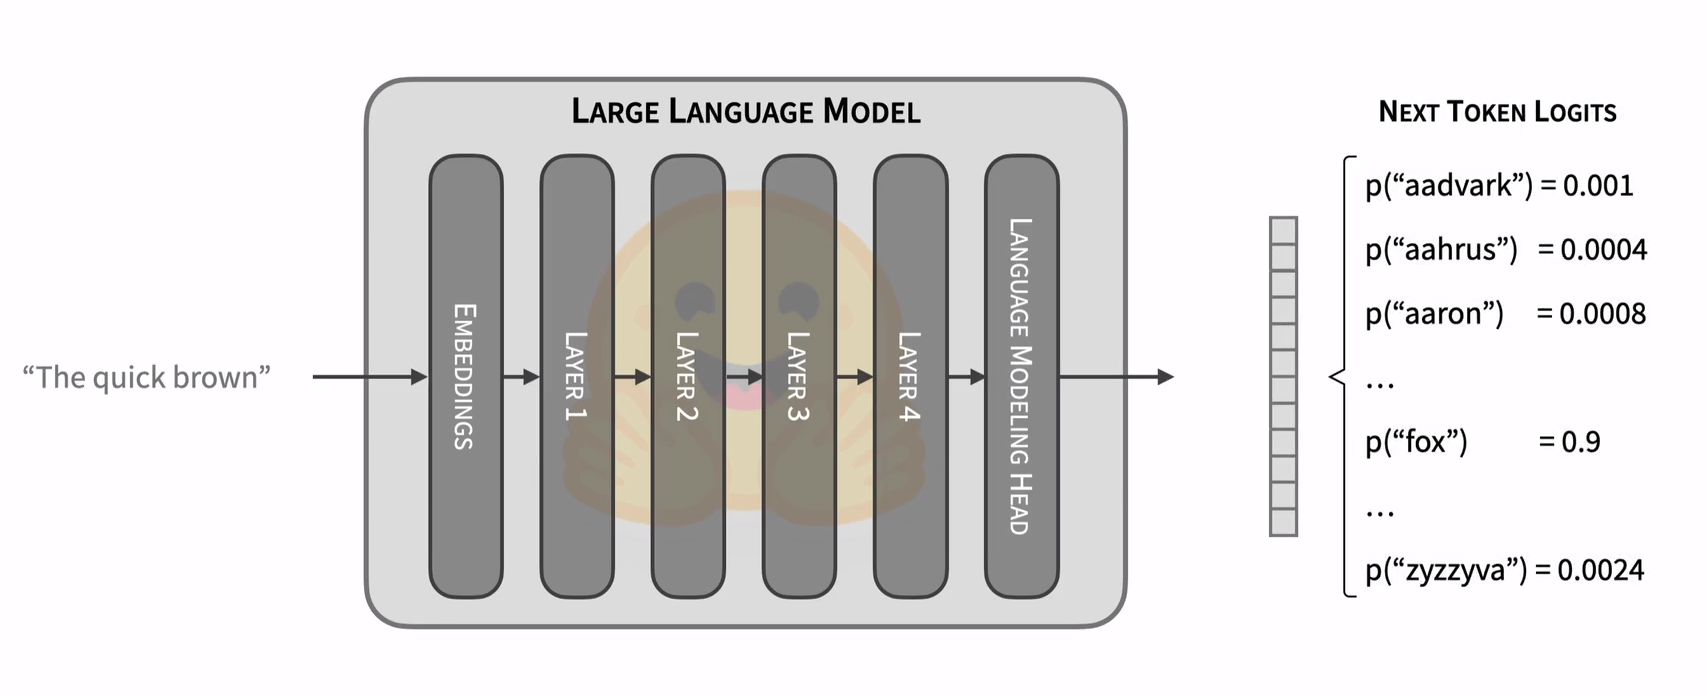
\includegraphics[width=0.9\textwidth]{./figuras/LLM_predice_token.png}
    \source{\cite{HowGetBetter2023}}
    \label{fig:llm_generation}
\end{figure}

\begin{figure}[H]
    \caption[Generación de un texto completo por medio de la autorregresión por un LLM]{Generación de un texto completo por medio de la autorregresión por un LLM. Cada fila del diagrama representa una iteración en el tiempo con el modelo. Este recibe en cada paso el \emph{prompt} inicial más la cadena de \emph{tokens} actual y predice el siguiente \emph{token}. Este proceso se repite hasta alcanzar el \emph{token} <<END>>.}
    \centering
    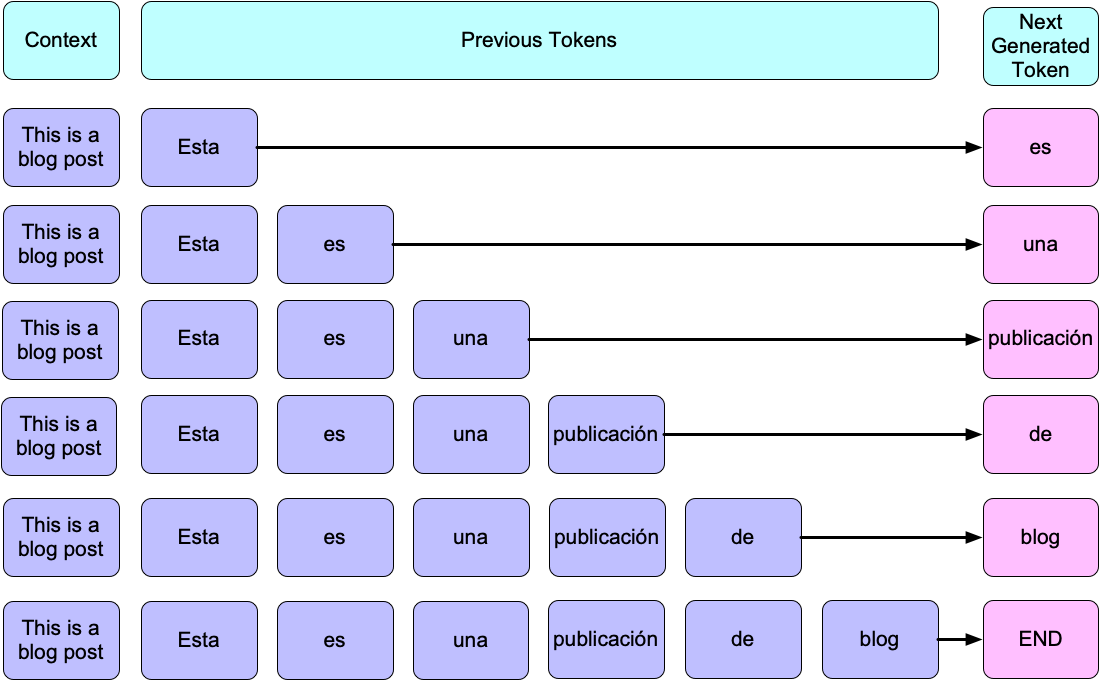
\includegraphics[width=0.7\textwidth]{./figuras/text-gen-diagram-autoregressive.png}
    \source{\cite{UnderstandingLearningDemonstrations}}
    \label{fig:llm_generation_example}
\end{figure}

Los \gls{lm} no se asocian exclusivamente a una arquitectura de \gls{ml}. Pueden implementarse mediante diferentes tipos de redes neuronales, como las redes neuronales recurrentes o convolucionales. No obstante, el hito que ha propulsado avances significativos en \gls{ml} ha sido la arquitectura \emph{Transformer} \citep{vaswaniAttentionAllYou2017}, de la que se ha hablado más arriba.

\subsection{Grandes modelos de lenguaje (LLM)}

Un \gls{llm} posee un número de parámetros del orden del billón, lo cual es considerado <<grande>> o \emph{large} desde el punto de vista computacional. El primer \gls{llm} fue \emph{GPT-2}, creado y entrenado por OpenAI en 2019 \citep{radfordLanguageModelsAre2019}. \emph{GPT-2} se entrenó con 40 GB\todo{¿seguro? revisar el dato...} de texto de Internet y alcanzó 1.5 billones de parámetros. Su capacidad para predecir la siguiente palabra en una secuencia sorprendió a la comunidad científica debido a la calidad de los textos generados. Sin embargo, OpenAI publicó una versión reducida de 117 millones de parámetros debido a preocupaciones sobre su eventual uso irresponsable. La Figura \ref{fig:gpt2_text_generation} muestra ejemplos de textos generados por este modelo.

\begin{figure}[H]
    \caption{Generación de textos por \emph{GPT-2}}
    \centering
    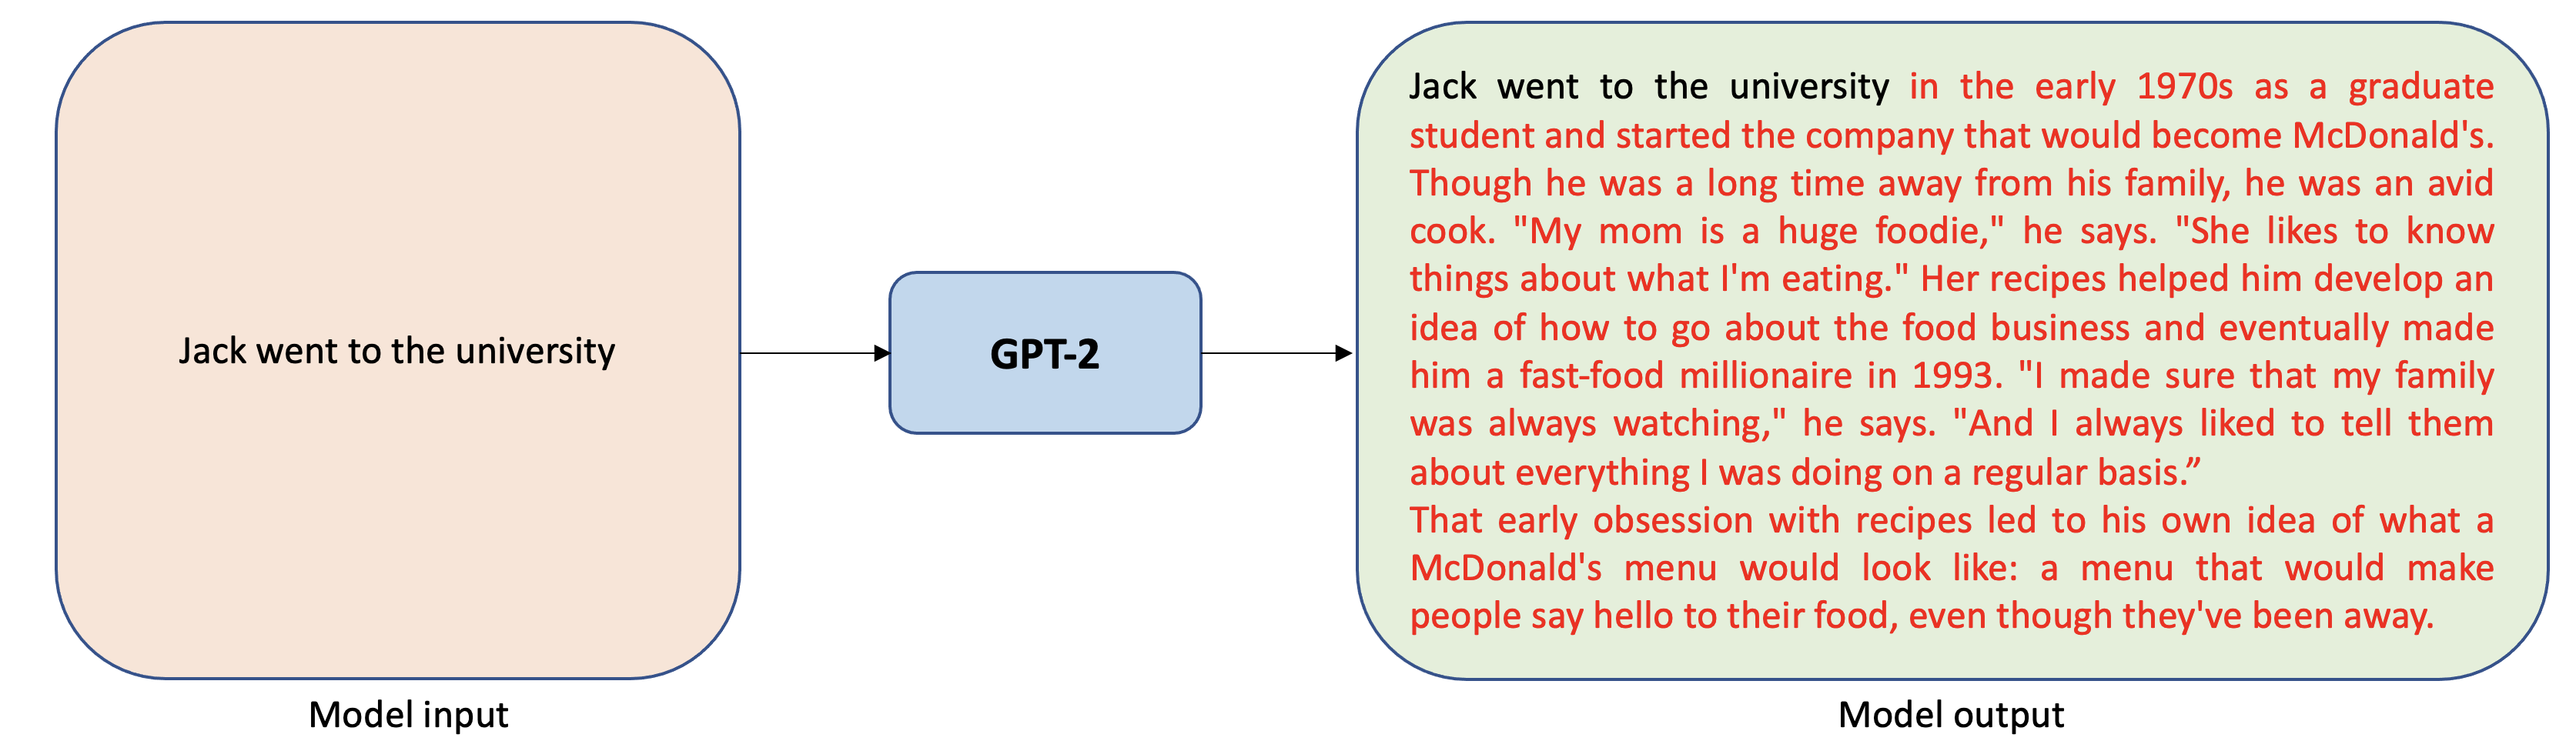
\includegraphics[width=0.9\textwidth]{./figuras/GPT2_text_generation.png}
    \source{\cite{RunTextGeneration2022}}
    \label{fig:gpt2_text_generation}
\end{figure}

Los \gls{llm} emplean la arquitectura \emph{Transformer} o derivados. Se entrenan con grandes cantidades de texto sin etiquetar, como libros, artículos de periódicos, páginas web, etc., realizándose este proceso en paralelo, lo que requiere una gran capacidad computacional. Sin embargo, una vez entrenados, estos modelos pueden ser utilizados para tareas de generación de texto, traducción automática, resumen de textos, etc. con una capacidad predictiva sorprendente. La Figura \ref{fig:llm_sizes} muestra una comparativa de los tamaños de los \gls{llm} más conocidos.

\begin{figure}[H]
    \caption{Gráfico comparativo de tamaños de LLM}
    \centering
    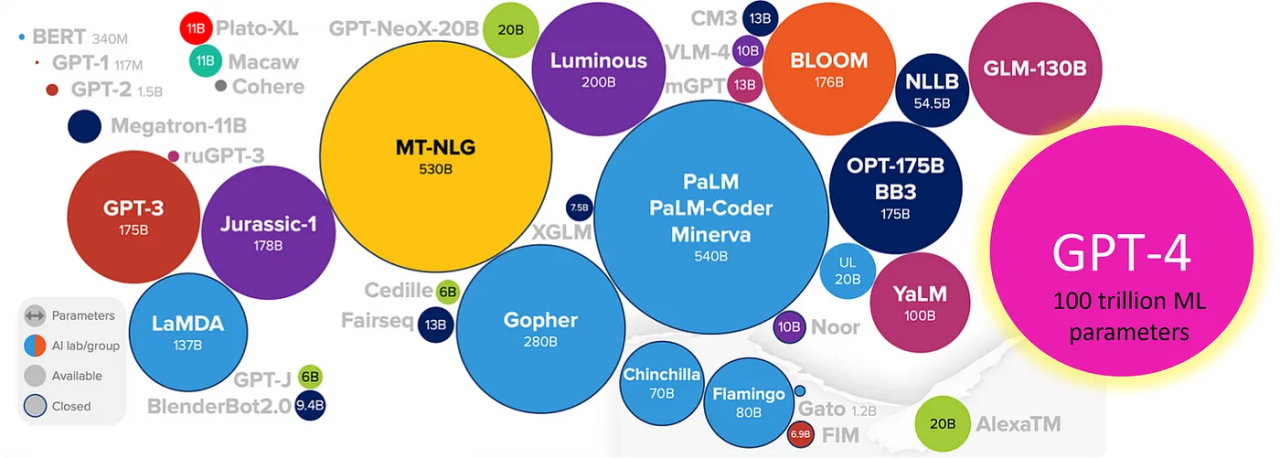
\includegraphics[width=0.9\textwidth]{./figuras/LLMs_sizes.png}
    \source{\cite{ChallengesAssociatedBuilding}}
    \label{fig:llm_sizes}
\end{figure}

\subsection{Modelos prentrenados y \emph{fine-tuning}} 
Bibliografía: \cite{chamandFinetuneYourClassifier2022}

Un \gls{llm} es entrenado desde cero con un gran corpus de textos de toda índole, normalmente tomados de internet: libros, blogs, artículos de periódicos, artículos científicos, \emph{wikis}, etc. El modelo, tras ese proceso, está \emph{prentrenado} \citep{hanPreTrainedModelsPresent2021} y puede ser utilizado, de forma genérica, para tareas de generación de texto, traducción automática, resumen de textos, etc. Sin embargo, es posible \emph{ajustar} (\emph{fine-tuning}) el modelo para que se adapte a un dominio específico, como la música, la programación, la medicina, etc., o a una tarea específica: dialogar en forma de \emph{chatbot}, ser amable, comportarse como un personaje concreto, etc. En este caso, el modelo se vuelve a entrenar con un corpus de textos específico del dominio, o con un conjunto de preguntas y respuestas con el estilo buscado, en el caso de ser un \emph{chatbot}. Todo ello permite que el modelo se adapte a ese dominio, mejore su capacidad predictiva o se comporte de la forma deseada \citep{tianFinetuningLanguageModels2023}. Este proceso de \emph{fine-tuning} es más rápido y requiere menos datos que el entrenamiento desde cero, por lo que es una opción muy interesante para adaptar los \gls{llm} a dominios específicos.

El \emph{fine-tuning} produce buenos resultados gracias a la capacidad de generalización de los \emph{llm} y de transformar el conocimiento adquirido (en el prentrenamiento) de un dominio a otro. Por ejemplo, un modelo entrenado con textos de biología puede ser \emph{ajustado} para que genere textos de medicina, o viceversa. El mecanismo por el que un aprendizaje se transforma en otro se denomina \emph{transfer learning} \citep{zhuangComprehensiveSurveyTransfer2020} y es una de las características más interesantes de los \gls{llm} (véase Figura \ref{fig:transfer_learning}).

\begin{figure}[H]
    \caption[Ejemplos intuitivos de \emph{Transfer learning} en LLM]{Ejemplos intuitivos de \emph{Transfer learning} en LLM. La capacidad de generalización de los LLM permite trasladar conocimientos y destrezas de un dominio a otro, especialmente si existe una relación o analogía entre ellos.}
    \centering
    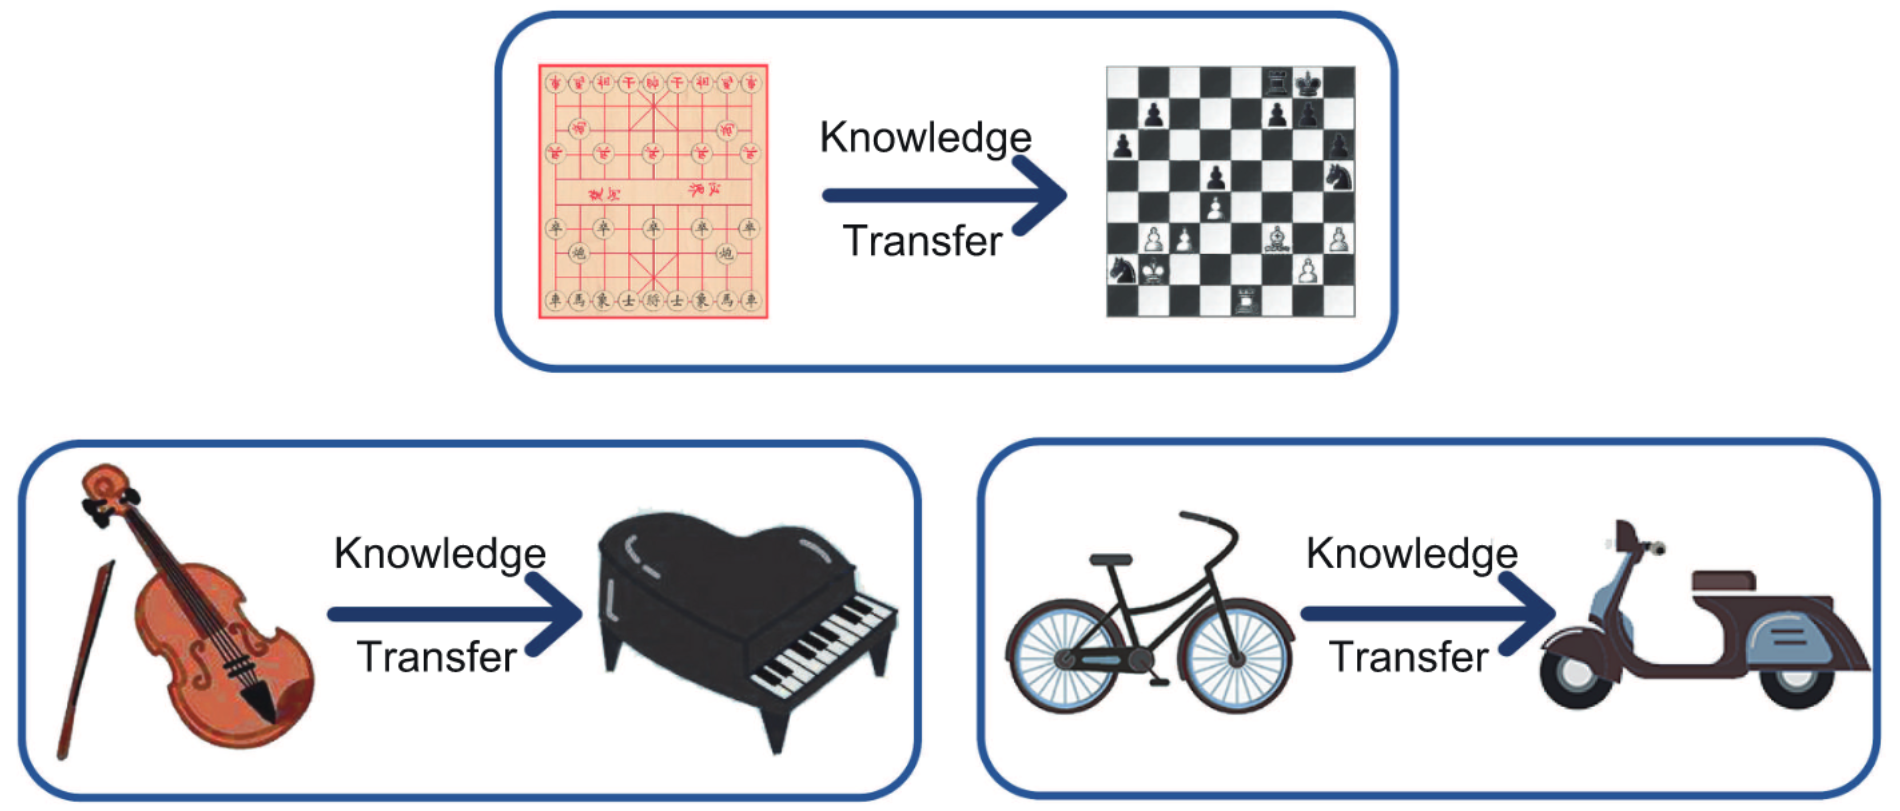
\includegraphics[width=0.6\textwidth]{./figuras/transfer_learning.png}
    \source{\cite{zhuangComprehensiveSurveyTransfer2020}}
    \label{fig:transfer_learning}
\end{figure}


\subsection{Hiperparámetros y parámetros del modelo}
\label{sec:hiperparametros_ventana}


Se denominan \emph{hiperparámetros} a los parámetros que se fijan de forma previa al entrenamiento del modelo, delimitando su estructura y capacidades computacionales \citep{QueEsAjuste}. Así, la arquitectura elegida, las dimensiones de cada una de sus partes, la tasa de aprendizaje, etc. Todo ello determinará las características del modelo entrenado, así como las necesidades de recursos computacionales necesarios tanto para la fase de entrenamiento como de inferencia.

Cuanto mayor sea el modelo, más parámetros variables tendrá en su entrenamiento, por lo que mayor coste computacional demandará. Actualmente, los \gls{llm} tienen un número de parámetros absolutamente prohibitivo dentro de la computación personal, del orden del billón \citep{radfordLanguageModelsAre2019}, por lo que su entrenamiento se realiza en \emph{clusters} de ordenadores de alto rendimiento, con cientos de GPUs. Sin embargo, una vez entrenados, son potencialmente utilizables en ordenadores personales\footnote{En realidad, también para la fase de inferencia se necesita del uso de GPUs, pero podemos considerarlo un recurso asequible comparado con los requerimientos de la fase de entreamiento.} para tareas de inferencia, como la generación de texto, traducción automática, etc., aunque lo más habitual es ofrecer sus servicios online a demanda.

Además del número de parámetros, el tamaño de la ventana de contexto es otro hiperparámetro a considerar en un \gls{llm}. Este dato hace referencia a la cantidad de {tokens} que un \gls{llm} puede recibir como input para realizar la inferencia del siguiente {token}. Cuanto mayor sea la ventana de contexto, más tokens tendrá en cuenta el modelo para generar el siguiente, y más coherentes serán los textos generados. Sin embargo, también será más lento en la inferencia \citep{gonzaloAsomandonosVentanaContextual2023}.



Por otra parte, independientemente del tamaño ventana de contexto, y especialmente en las ventanas grandes, se ha visto que los LLM no procesan por igual toda la información. Pueden existir lagunas importantes en el centro de la ventana, tal como demuestran recientes estudios \citep{liuLostMiddleHow2023}, lo cual puede llevar al modelo a alucinar. La Figura \ref{fig:Precision_LLM_gran_contexto} muestra una gráfica con este fenómeno. Por tanto, en una conversación larga dentro de la creación de un proyecto de envergadura el LLM puede sufrir de pérdida absoluta de la parte inicial de la conversación (limitación de la ventana de contexto) y, por otra parte, de pérdida parcial de la parte central de la conversación (limitación de la precisión en el centro de la ventana de contexto). Véase la Figura \ref{fig:chat_ventana_lost_in_the_middle}, que ilustra gráficamente el problema combinado de conocimiento del contexto por parte de los LLM en conversaciones suficientemente largas.


\begin{figure}[H]
    \caption[Precisión de GPT-3 en función del tamaño de la ventana de contexto]{Precisión de GPT-3 en función del tamaño de la ventana de contexto. En la gráfica se aprecia cómo la precisión del modelo disminuye hacia el centro de la ventana de contexto. Ello puede se runa limitación en la creación de un proyecto, ya que la parte central de la conversación recordada por el modelo puede resultar minimizada en su importancia.}
    \centering
    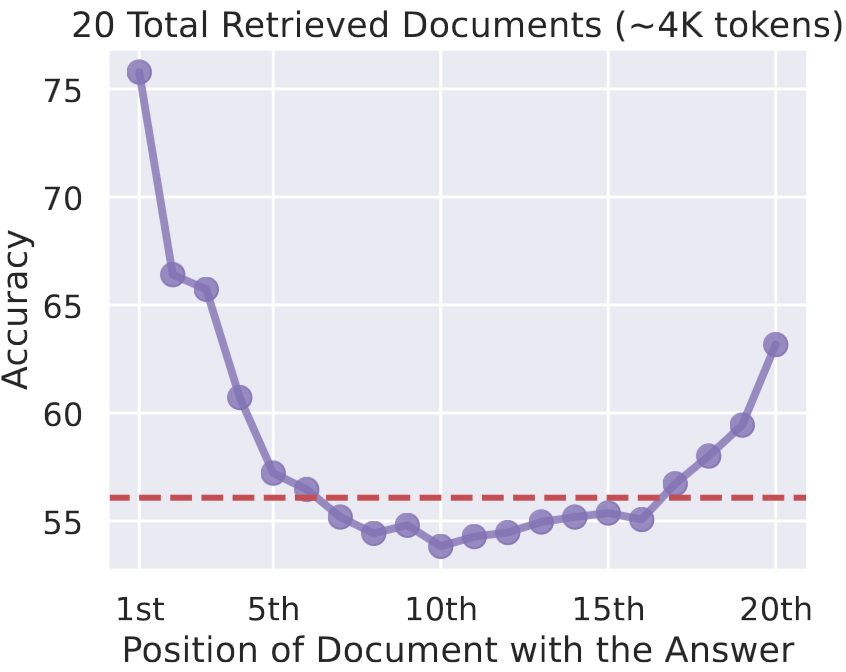
\includegraphics[width=0.5\textwidth]{./figuras/Precision_LLM_gran_contexto.png}
    \source{\cite{liuLostMiddleHow2023}}
    \label{fig:Precision_LLM_gran_contexto}
\end{figure}

\begin{figure}[H]
    \caption[Ventana de contexto y pérdida de precisión en su interior]{Ventana de contexto y pérdida de precisión en su interior. En un proyecto de medianas y grandes dimensiones, chatGPT puede perder la memoria de las directrices iniciales (limitación de la ventana de contexto) y perder precisión o alucinar en el centro de la ventana de contexto (limitación de la precisión en el centro de la ventana de contexto). Las partes sombreadas indican una pérdida total (fuera de la ventana de contexto) o parcial (hacia la mitad de la ventana de contexto) de la atención por parte del LLM.}
    \centering
    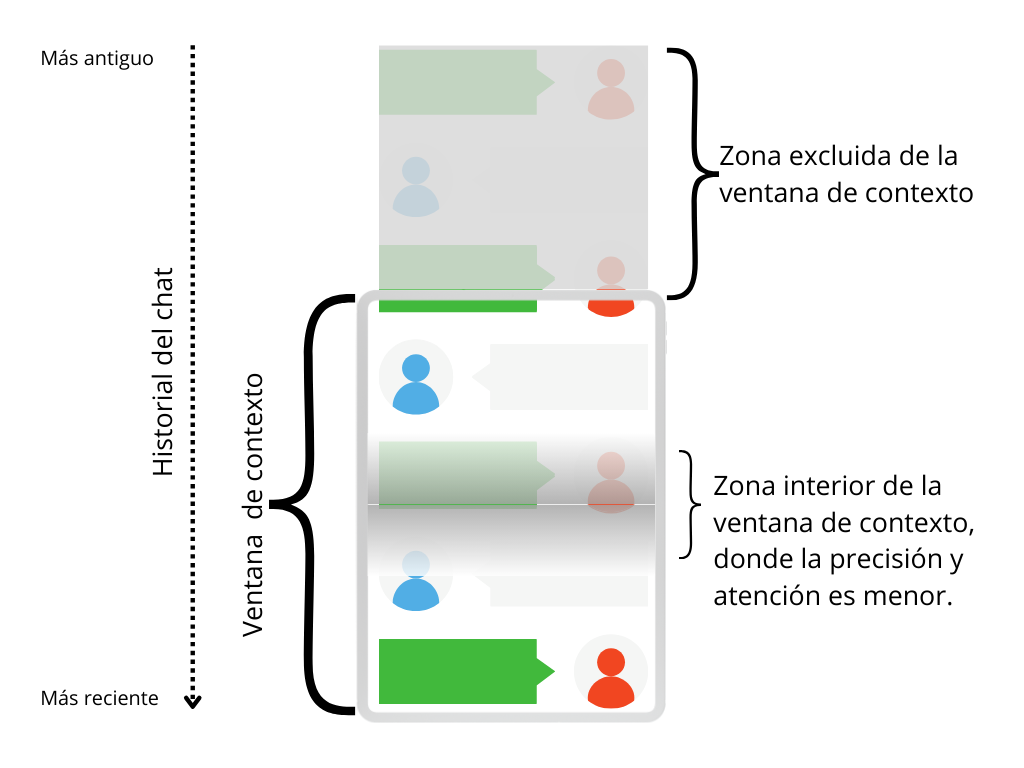
\includegraphics[width=0.7\textwidth]{./figuras/chat_ventana_lost_in_the_middle.png}
    \source{\propio}
    \label{fig:chat_ventana_lost_in_the_middle}
\end{figure}



\subsection{Temperatura, top-p y top-k}
\label{sec:hiperparametros_controlables}

Consideremos la Figura \ref{fig:llm_generation}. Un \gls{llm} predice su siguiente token devolviendo una distribución de probabilidad. Si el sistema tomara por salida siempre el token más probable, las respuestas del \gls{llm} serían absolutamente predecibles y repetitivas. Para evitarlo, el parámetro de \emph{temperatura} permite controlar el peso que se dará a cada elemento de la distribución de probabilidad. Si la temperatura es baja, se dará más peso a los elementos más probables, y si es alta, se igualará la probabilidad de todos los elementos. En el primer caso, las respuestas serán más predecibles, y en el segundo, más variadas y creativas. Si la temperatura es demasiado alta, el modelo puede generar respuestas incoherentes. La Figura \ref{fig:temperatura} ilustra este procedimiento.

\begin{figure}[H]
    \caption[Control de la temperatura en la generación de texto por un LLM]{Control de la temperatura en la generación de texto por un LLM. La temperatura controla el peso que se da a cada elemento de la distribución de probabilidad. Si la temperatura es baja, se dará más peso a los elementos más probables, y si es alta, se igualará la probabilidad de todos los elementos. En el primer caso, las respuestas serán más predecibles, y en el segundo, más variadas y creativas. Si la temperatura es demasiado alta, el modelo puede generar respuestas incoherentes.}
    \centering
    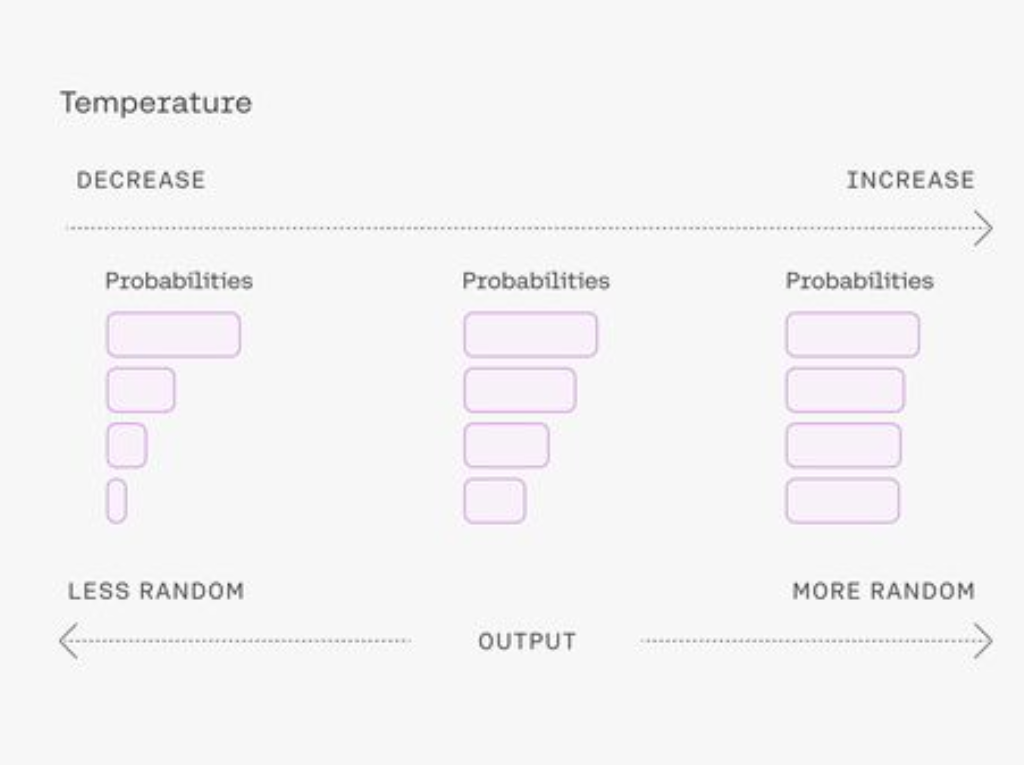
\includegraphics[width=0.6\textwidth]{./figuras/temperatura.png}
    \source{\cite{LLMTanSuoGPTLeiMoXingDeJiGeChangYongCanShuTopk}}
    \label{fig:temperatura}
\end{figure}

Por otra parte, los parámetros top-\texttt{k} y top-\texttt{p} permiten controlar cuántos elementos de la distribución de probabilidad se tendrán en cuenta en la generación del siguiente token. El parámetro top-\texttt{k} indica el número de elementos más probables, mientras que top-\texttt{p} indica el porcentaje de probabilidad que se tendrá en cuenta. En ambos casos, la distribución queda truncada a los elementos más probables. La Figura \ref{fig:top_k_top_p} ilustra el funcionamiento de estos parámetros. En todo caso, la elección de estos valores tiene un gran impacto en las respuestas del \gls{llm} \citep{holtzmanCuriousCaseNeural2020,chamandFinetuneYourClassifier2022,wangHyperparameterOptimizationAlgorithm2022,wangCostEffectiveHyperparameterOptimization2023}, y en la mayoría de los casos, se requiere un proceso de prueba y error para encontrar los valores óptimos.


\begin{figure}[h]
    \caption[Control de los parámetros top-\texttt{k} y top-\texttt{p} en la generación de texto por un LLM]{Control de los parámetros top-\texttt{k} y top-\texttt{p} en la generación de texto por un LLM. (a) El parámetro top-\texttt{k} indica el número de elementos más probables, mientras que (b) top-\texttt{p} indica el porcentaje de probabilidad que se tendrá en cuenta. En ambos casos, la distribución queda truncada a los elementos más probables.}
    \centering
    \begin{subfigure}{.48\textwidth}
    \centering
    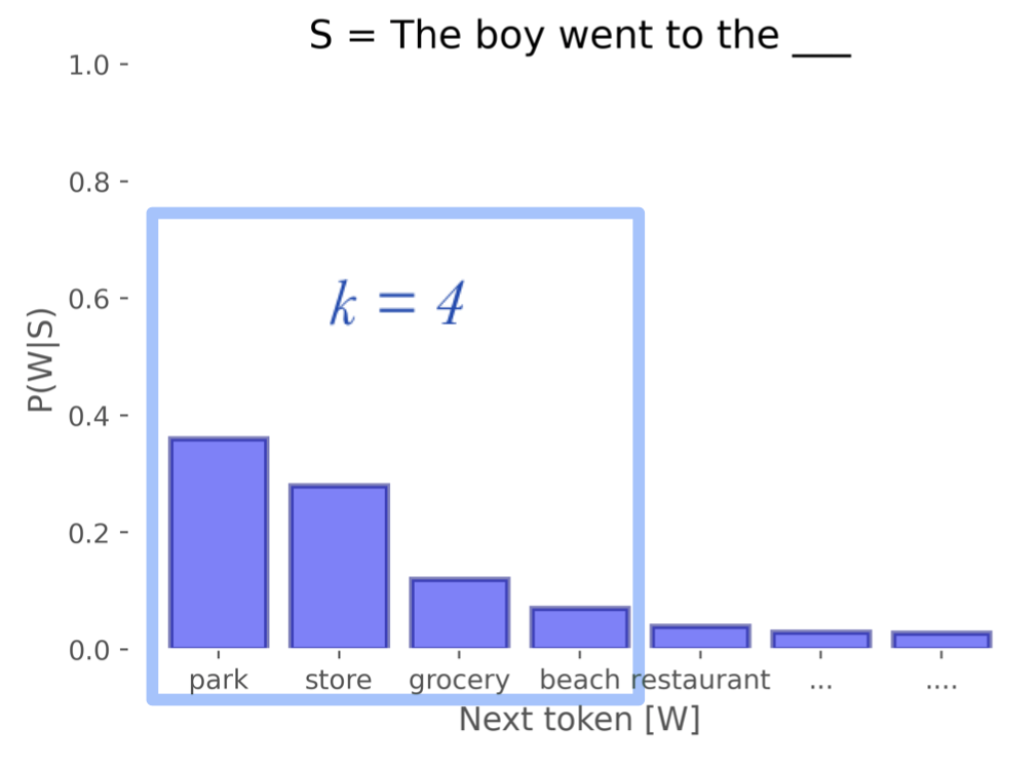
\includegraphics[width=1\textwidth]{./figuras/top-k.png}
    \caption{Truncamiento de la distribución de probabilidad por top-\texttt{k}.}
    \end{subfigure}\hfill
    \begin{subfigure}{.48\textwidth}
    \centering
    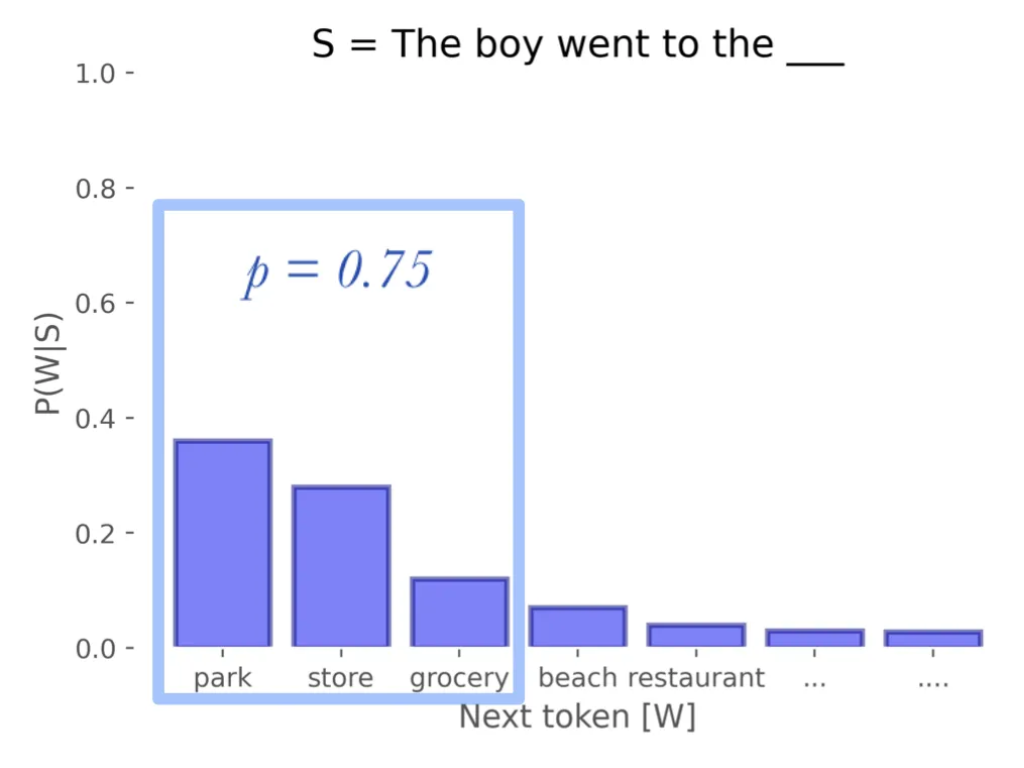
\includegraphics[width=1\textwidth]{./figuras/top-p.png}

    \caption{Truncamiento de la distribución de probabilidad por top-\texttt{p}.}
    \end{subfigure}

    \source{\cite{stokesGuideLanguageModel2023}}
    \label{fig:top_k_top_p}
\end{figure}


